\chapter{Preliminaries}
\label{chap:prelim}
%\setlength{\parskip}{1.5mm}
%\setlength{\baselineskip}{1.4mm}

\section{Present-day Cryptography}
Cryptography is the  study and practice of techniques for secure data transfer over insecure channels in presence of unauthorized users, usually called adversaries. Prior to modern age, cryptography was most exclusively referred to as encryption, i.e. the process of converting data from readable state to apparent noise.

Most of the present-day encryption algorithms are based on overlapping theory of mathematics and computer science. These are largely designed around `trap-door functions', i.e. problems with sufficient computational hardness. These problems can be theoretically solved, but is is not possible to do within reasonable time and with the resources that are usually at disposal.

Advances in mathematics such as improved algorithms on the integer factorization problem and discrete logarithm problem and availability of more computational power require these methods to adapt with time. Most of the algorithms can, however, be made secure against these advancements just by increasing the key-length.

\section{Shor's Algorithm}
Published in 1995 and named after it's formulator, Shor's algorithm, is a quantum algorithm for finding the prime factors of any given integer N.

The importance of Shor's algorithm lies in it's ability to find the prime factors of an integer in polynomial time, in comparison to the most efficient classical algorithms known, such as general number field sieve, which takes sub-exponential time. This is possible to due to efficiency of quantum fourier transform and modular exponentiation by repeated squaring.

\section{Shor's Algorithm \& Present Encryption Methods}
All of the popular cryptographic algorithms rely on one of the three hard problems - integer factorization problem, the discrete logarithm problem or the elliptic-curve discrete logarithm problem. These problems were viewed as important because many cryptography systems rely upon the difficulty of factoring large numbers. If an efficient method of factoring large numbers can be implemented, most of the encryption schemes would be next to worthless to protect their data. 

With Shor's algorithm, these can be be solved in reasonable polynomial time. This implies that, with a quantum computer having sufficient number of qubits, Shor's algorithm can be used to break the public-key cryptography schemes including RSA. However, the experimental quantum computers available today succumb to noise and decoherence problems, hence, cannot be used to break current encryption schemes.

\section{Post-Quantum Cryptography}
Post-Quantum Cryptography refers to the study of classical encryption schemes that are considered to be secure against an attack by quantum computers. As discussed above, most of the popular encryption methods can be efficiently broken using a sufficiently powerful hypothetical quantum computer. Thus, scientists are preparing methods to secure data against attacks when quantum computing becomes much more powerful.

Daniel J. Bernstein[11] lists the following important classes of cryptographic methods beyond RSA, DSA and ECRSA -
\begin{description}[align=left, style=multiline,leftmargin=4 cm]
\item [Hash-based - ] This includes Merkle's hash-tree public-key signature system, building upon the one-message idea.
\item [Code-based - ] An example is McEliece's hidden-Goppa-code public-key encryption system.
\item [Lattice-based - ] The most popular example that garnered most of the interest is Hoffstein-Pipher-Silverman NTRU public-key-encryption system.
\item [Multivariate quadratic equation based- ] One of the examples is Patarin's {\em HFEv} public-key-signature system originally proposed by Matsumoto and Imai.\\
\item [Secret-key based - ] The prominent example is the DaemenRijmen
{\em Rijndael} cipher which was later named AES (Advanced Encryption Standard).
\end{description}

\begin{figure}[H]
\centering
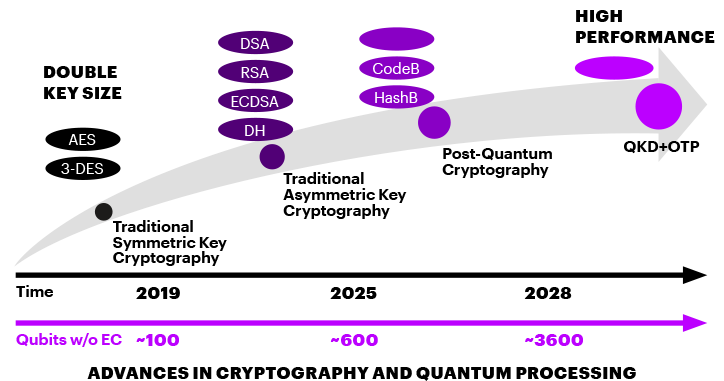
\includegraphics[width=14cm]{timeline.png}
\caption{Timeline for Cryptography \& Quantum Processing}\label{fig:timeline}
\end{figure}


%All of these encryption methods are considered to be resistant to both classical and %quantum computing. These schemes are built around cryptographic primitives for which no %efficient algorithm has been found yet, either for quantum or for classical computers.


\section{Chaos based Cryptography}
Apart from the popular post-quantum cryptographic methods, a new method of constructing cryptosystems utilising the non-predictability property of discrete chaotic systems has become somewhat noteworthy from practical perspectives. This type of systems are based on the characteristics of chaos, which are sensitivity of parameters, sensitivity of initial points, and randomness of sequences obtained by iterating a chaotic map. A ciphertext is obtained by the iteration of an inverse chaotic map from an initial point denoting a plaintext. 

If the number of iterations is large enough, the randomness of the encryption and the decryption functions would be so large that attackers would be unable to break this cryptosystem by statistical characteristics. Hence, nonlinear dynamic systems with chaos are generally viewed to be good candidates for constructing such encryption-decryption algorithms. Most of these methods have been used in the development of symmetric ciphers for encryption of 2D images.

\begin{figure}[H]
\begin{subfigure}{0.5\textwidth}
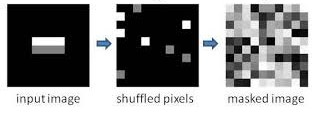
\includegraphics[width=1\linewidth]{image_chaos0.jpg}
\caption{Image Encryption using 1D Chaotic Map}\label{fig:image_chaos0}
\end{subfigure}
\begin{subfigure}{0.5\textwidth}
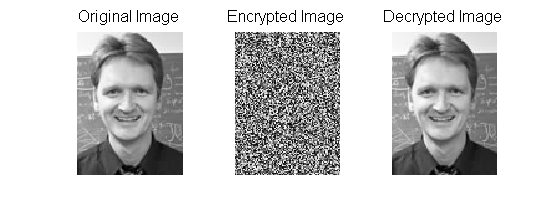
\includegraphics[width=1\linewidth]{image_chaos.png}
\caption{Chaos based Image Encryption}\label{fig:image_chaos}
\end{subfigure}
\caption{Chaos based Cryptography}\label{fig:image0}
\end{figure}

\section{Field Programmable Gate Array}
A field programmable gate array is a set (array) of reconfigurable gates that can implement both sequential and combinational logic including multi-level logic functions.

FPGAs are built in form of an array of configurable logic blocks (CLBs). Each of these CLBs can be programmed to perform a logic function and then connected to each other through a hierarchy of interconnects (routing channels) to form a complex logic. FPGA also has a set of I/O elements for interfacing with external devices such as flash memories and network ports.

The structure of CLBs varies with model and manufacturers, but all of them share a lot of similarity. Figure 2.3 shows the structure of Cyclone IV CLB, consisting of a 4-input LUT and a flip-flop. By loading appropriate values, the LUT can be programmed to perform any 4-input function. Further, the choice of multiplexer select signals determines how the data is routed through LUT to the neighbouring LEs and IOEs. The LUT output either goes directly to the LE output for combinational logic, or it can be routed through the register for sequential logic.
\begin{figure}[H]
\centering
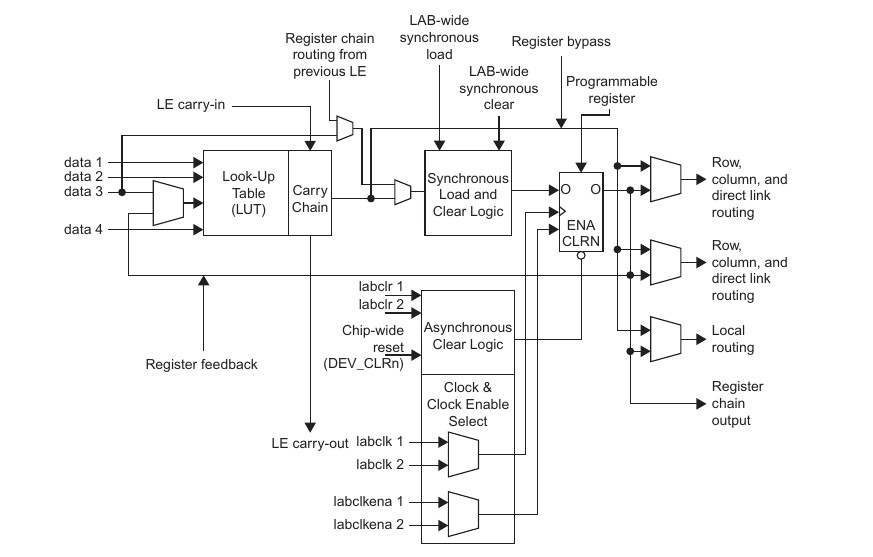
\includegraphics[width=13cm]{fpga.jpg}
\caption{FPGA CLB Structure}\label{fig:fpga}
\end{figure}

An engineer programs the logic using Hardware Description Language (HDLs) such as VHDL or Verilog. A synthesis is then used to generate a gate-level netlist. An implementation tool then determines how the CLBs and routing channels should be configured to perform the specified function and generates a bitstream that can be loaded into a FPGA.
